\RequirePackage{shellesc}
\immediate\write18{cd ..; tex spath3_code.dtx}
\documentclass{article}
\usepackage[svgnames]{xcolor}
\RequirePackage[enable-debug]{expl3}
\ExplSyntaxOn
\debug_on:n {check-declarations, deprecation}
\ExplSyntaxOff
\usepackage{tabularx}
\usepackage{tikz}
\usetikzlibrary{spath3,intersections,patterns,hobby}

\makeatletter
\def\showpath{%
  \def\pgfqpoint##1##2{(##1, ##2)}%
  \def\pgfsyssoftpath@movetotoken##1##2{%
    M\{##1\}\{##2\}
  }%
  \def\pgfsyssoftpath@linetotoken##1##2{%
    L\{##1\}\{##2\}
  }%
  \def\pgfsyssoftpath@curvetotoken##1##2{%
    C\{##1\}\{##2\}
  }%
  \def\pgfsyssoftpath@curvetosupportatoken##1##2{%
    Ca\{##1\}\{##2\}
  }%
  \def\pgfsyssoftpath@curvetosupportbtoken##1##2{%
    Cb\{##1\}\{##2\}
  }%
  \def\pgfsyssoftpath@closepathtoken##1##2{%
    Z\{##1\}\{##2\}
  }%
}
\makeatother

% Note: this was for a previous version and doesn't work with the
% current one, but it might be useful to adapt it to the current
% version so I'm keeping it around to remember what it originally
% looked like.

\newcommand\displaypath[1]{%

Displaying path information for: #1

\begin{tabularx}{\textwidth}{r@{:\hskip\arraycolsep}>{\raggedright\arraybackslash}X}
Length & \SPathInfo{#1}{length} \\
Real length & \SPathInfo{#1}{reallength} \\
Number of components & \SPathInfo{#1}{numberofcomponents} \\
Initial point & \showpath\SPathInfoInto{#1}{initialpoint}{\stuff}\expandafter\pgfqpoint\stuff \\
Final point & \showpath\SPathInfoInto{#1}{finalpoint}{\stuff}\expandafter\pgfqpoint\stuff \\
Initial action & \texttt{\showpath\SPathInfo{#1}{initialaction}} \\
Final action & \texttt{\showpath\SPathInfo{#1}{finalaction}} \\
Path & \texttt{\showpath\SPathInfo{#1}{path}} \\
Reverse path & \texttt{\showpath\SPathInfo{#1}{reversepath}} \\
Min bb & \showpath\SPathInfoInto{#1}{minbb}{\stuff}\expandafter\pgfqpoint\stuff \\
Max bb & \showpath\SPathInfoInto{#1}{maxbb}{\stuff}\expandafter\pgfqpoint\stuff 
\end{tabularx}%
}

\makeatletter
\tikzset{
  show last coords/.code={
    \edef\tikz@last@coords{(%
      \the\tikz@lastx,
      \the\tikz@lasty), (%
      \the\tikz@lastxsaved,
      \the\tikz@lastysaved), (%
      \the\tikz@lastmovetox,
      \the\tikz@lastmovetoy)%
    }%
    \show\tikz@last@coords
  },
  show tikz timer/.code={
    \show\tikz@timer
  }
}
\makeatother

\ExplSyntaxOn

\DeclareDocumentCommand\SPathPoint {m m}
{
  \spath_get_point_at:nnN {#1} {#2} \l__tmpa_tl
  \tl_show:N \l__tmpa_tl
}

\ExplSyntaxOff
\begin{document}

\begin{tikzpicture}
\path[spath/save=a] (0,0) -- node[pos=.5,auto] {\(a\)}
 ++(2,0) to[out=0,in=-90] node[pos=.5,auto] {\(b\)} ++(2,2) to[out=90,in=0] node[pos=.5,auto] {\(c\)} ++(-2,2)
;
\draw[spath/restore=a]
node[pos=.16,auto,swap] {\(a\)}
node[pos=.5,auto,swap,sloped] {\(b\)}
node[pos=.84,auto,swap,sloped,allow upside down] {\(c\)}
;

\draw (0,-1) -- ++(3,-1) [spath/append=a]
node[pos=.16,auto,swap] {\(a\)}
node[pos=.5,auto,swap,sloped] {\(b\)}
node[pos=.84,auto,swap,sloped,allow upside down] {\(c\)}
;
\end{tikzpicture}


\begin{tikzpicture}
\begin{scope}[scale=.5, rotate=30, xscale=2, shift={(3,-1)}]
\path
(0,0) node[circle,fill] {}
(2,1) node[circle,fill] {}
++(2,0) node[circle,fill] {}
+(0,1) node[circle,fill] {}
+(0,3) node[circle,fill] {}
+(1,0) node[circle,fill] {}
;
\draw[spath/save global=b, line width=5pt, orange] (2,1) -- ++(1,1) -- +(1,-1) [show last coords];
\end{scope}
\path
(spath cs:b 1) node[circle,fill=blue] {}
+(0,1) node[circle,fill=blue] {}
+(0,3) node[circle,fill=blue] {}
+(1,0) node[circle,fill=blue] {}
;

\tikzset{spath/show=b}
\draw[spath/restore=b,show last coords] -- +(0,1);
\tikzset{spath/show=b}
\begin{scope}[scale=3]
\draw[spath/restore=b,show last coords] -- +(0,1);
\end{scope}
\draw[spath/restore=b] to[out=-90,in=-90] +(1,0);
\draw[spath/restore=b] to[out=-90,in=-90] cycle;
\end{tikzpicture}


\begin{tikzpicture}[use Hobby shortcut]
\path[spath/save=figure8] ([closed]0,0) .. (1.5,1) .. (.5,2) .. (-.5,1) .. (.5,0) .. (0,-.5) .. (-.5,0) .. (.5,1) .. (-.5,2) .. (-1.5,1) .. (0,0);
\tikzset{spath/knot={figure8}{8pt}{2,4,6,8}}
\path (0,-.7);
\end{tikzpicture}


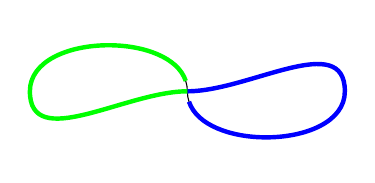
\begin{tikzpicture}
\path[spath/save=curve,draw] (0,0) to[out=-90,in=180] (2,0) to[out=0,in=90] (4,0) to[out=-90,in=-90] (2,0) to[out=90,in=90] cycle;
\tikzset{
  every spath component/.style={draw, ultra thick},
  curve component 1/.style={blue},
  curve component 2/.style={green},
  curve component 3/.style={orange},
  curve component 4/.style={magenta},
  curve component 5/.style={cyan},
  curve component 6/.style={green!50!black},
  curve component 7/.style={yellow!50!black},
  curve component 8/.style={red!50!black},
  curve component 9/.style={blue!50!black},
  spath/draft mode=true,
  spath/knot={curve}{8pt}{},
}
\end{tikzpicture}

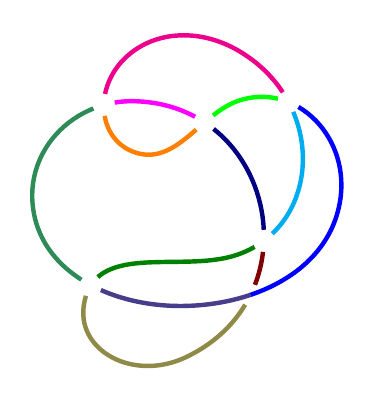
\begin{tikzpicture}[use Hobby shortcut]
\path[spath/save=6-3,scale=1.3] ([closed]0,0) .. (1.5,1) .. (.5,2) .. (-.5,1.5) .. (-.5,2.5) .. (.5,2.5) .. (.5,.5) .. (-1,0) .. (0,-.5) .. (-.5,2) .. (-1.5,1) .. (0,0);
\tikzset{
  every spath component/.style={draw,ultra thick},
  6-3 component 1/.style={blue},
  6-3 component 2/.style={green},
  6-3 component 3/.style={orange},
  6-3 component 4/.style={magenta},
  6-3 component 5/.style={cyan},
  6-3 component 6/.style={green!50!black},
  6-3 component 7/.style={yellow!50!black},
  6-3 component 8/.style={red!50!black},
  6-3 component 9/.style={blue!50!black},
  6-3 component 10/.style={Fuchsia},
  6-3 component 11/.style={SeaGreen},
  6-3 component 12/.style={DarkSlateBlue},
  spath/draft mode=true,
  spath/knot={6-3}{8pt}{},%2,4,...,12}
}
\end{tikzpicture}

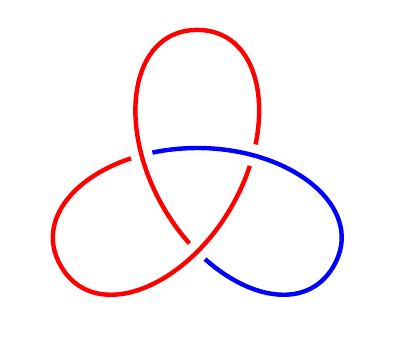
\begin{tikzpicture}[
  use Hobby shortcut,
  knot/.style 2 args={
    every #1 component/.style={ultra thick, draw, red},
    #1 component 1/.style={blue},
    spath/.cd,
    split at self intersections=#1,
    remove empty components=#1,
    insert gaps after components={#1}{8pt}{#2},
    spot weld=#1,
    render components=#1
  }
]
\path[spath/save=trefoil] ([closed]90:2) foreach \k in {1,...,3} { .. (-30+\k*240:.5) .. (90+\k*240:2) } (90:2);
\tikzset{knot={trefoil}{1,3,5}}
\end{tikzpicture}

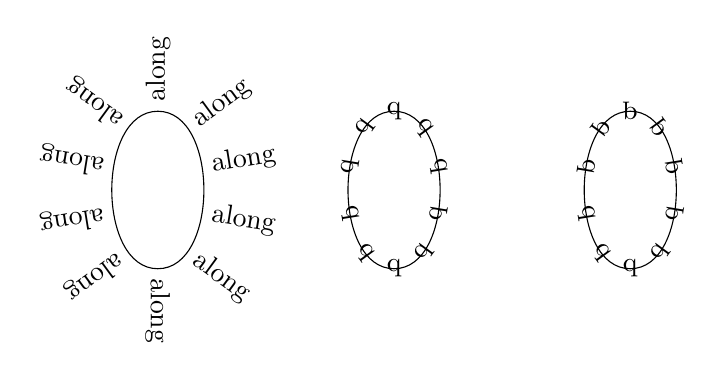
\begin{tikzpicture}
\draw[spath/save=oval] (0,0) to[out=0,in=0] (0,2) to[out=180,in=180] (0,0);
\foreach \k in {0,...,9} {
  \node[transform shape, allow upside down=false, spath/transform to={oval}{0.\k}, rotate=-90,right] {along};
}
\begin{scope}[xshift = 3cm]
\draw[spath/save=soval] (0,0) to[out=0,in=0] (0,2) to[out=180,in=180] (0,0);
\foreach \k in {0,...,9} {
  \node[transform shape, spath/upright transform to={soval}{0.\k}] {q};
}
\begin{scope}[xshift = 3cm]
\draw[spath/save=soval] (0,0) to[out=0,in=0] (0,2) to[out=180,in=180] (0,0);
\foreach \k in {0,...,9} {
  \node[transform shape, spath/transform to={soval}{0.\k}] {q};
}
\end{scope}
\end{scope}
\end{tikzpicture}



\begin{tikzpicture}
\draw[spath/save=oval] (0,0) to[out=0,in=0] (0,2) +(-1,0) to[out=180,in=180] (0,0);
\tikzset{spath/spot weld=oval}
\end{tikzpicture}

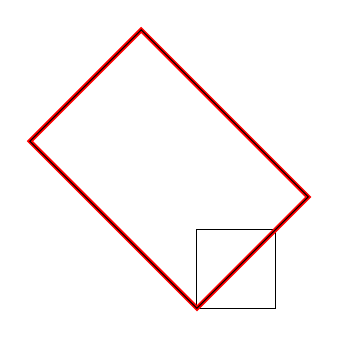
\begin{tikzpicture}
\draw[spath/save=tpath] (0,0) rectangle +(1,1);
\draw[rotate=45, xscale=2, yscale=3, ultra thick, red] (0,0) rectangle +(1,1);
\draw[
  spath/transform={tpath}{rotate=45, xscale=2, yscale=3},
  spath/restore={tpath}];
\end{tikzpicture}

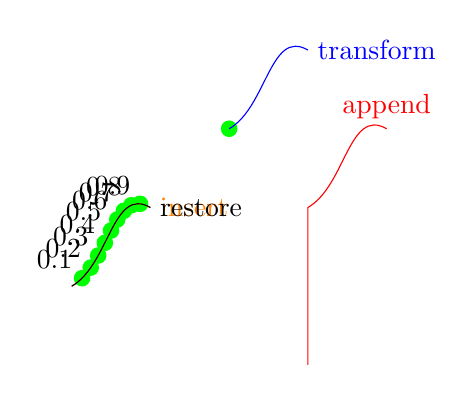
\begin{tikzpicture}
\path[spath/save=rpath] (0,0) to[out=30,in=150] (1,1);
\foreach \k in {1,...,9} {
  \fill[green] (spath cs:rpath 0.\k) circle[radius=3pt];
  \node[above left] at (spath cs:rpath 0.\k) {\(0.\k\)};
}
\fill[green] (2,2) circle[radius=3pt];
\draw[blue, spath/transform={rpath}{shift={(2,2)}}, spath/restore={rpath}] node[right] {transform};
\draw[orange] (3,0) [spath/insert={rpath}] node[right] {insert};
\draw[red] (3,-1) -- +(0,2) [spath/append={rpath}] node[above] {append};
\draw[spath/restore={rpath}] node[right] {restore};
\end{tikzpicture}

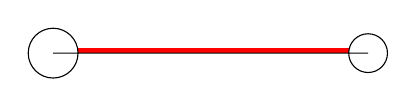
\begin{tikzpicture}
\path[spath/save=apath] (0,0) foreach \k in {1,...,4} { -- ++(1,0) +(0,0)};
\draw[
  spath/shorten at end={apath}{7pt},
  spath/shorten at start={apath}{9pt},
  spath/translate={apath}{0pt}{1pt},
  spath/restore=apath,
  ultra thick, red
];
\draw (0,0) circle[radius=9pt] [spath/insert=apath] circle[radius=7pt];
\end{tikzpicture}

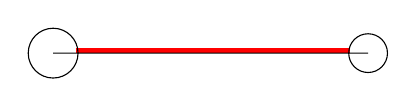
\begin{tikzpicture}
\path[spath/save=apath] (0,0) foreach \k in {1,...,4} { to[out=0,in=180] ++(1,0) +(0,0)};
\draw[
  ultra thick,
  red,
  spath/.cd,
  shorten at end={apath}{7pt},
  shorten at start={apath}{9pt},
  translate={apath}{0pt}{1pt},
  restore=apath,
];
\draw (0,0) circle[radius=9pt] [spath/insert=apath] circle[radius=7pt];
\end{tikzpicture}

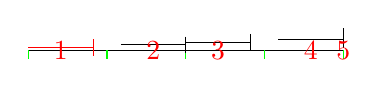
\begin{tikzpicture}
\draw[spath/save=npath] (0,0) foreach \k in {1,...,4} { -- ++(1,0) +(0,0)};
\draw[green] (0,0) -- +(0,-3pt) foreach \k in {1,...,4} { -- +(0,-3pt) ++(1,0)} -- +(0,-3pt);
%\expandafter\show\csname tikz@intersect@path@name@npath\endcsname
\tikzset{
  spath/.cd,
  insert gaps after components={npath}{10pt}{1,3},
  get components of={npath}\components,
}
%\show\components

\tikzset{
  path 1/.style={
    red,
  },
}

\foreach[count=\k] \cpt in \components {
  \path[
    draw,
    path \k/.try,
    spath/.cd,
    translate=\cpt{0pt}{\k pt},
    restore=\cpt,
  ] +(0,3pt) -- +(0,-3pt);
  \node[text=red] at (spath cs:{\cpt} .5) {\(\k\)};
}
\end{tikzpicture}

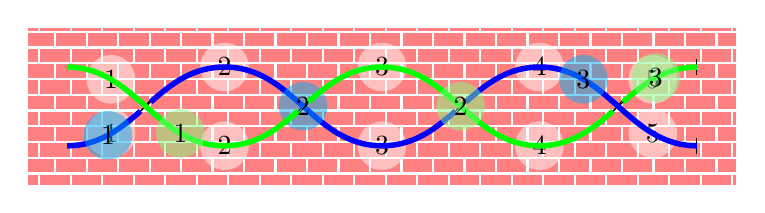
\begin{tikzpicture}[
  use Hobby shortcut,
]

\fill[red!50!white] (-.5,-.5) rectangle (8.5,1.5);
\fill[pattern=bricks, pattern color=white] (-.5,-.5) rectangle (8.5,1.5);

\path[spath/save=pathA] (0,0) to[out=0,in=180] ++(2,1) to[out=0,in=180] ++(2,-1)  to[out=0,in=180] ++(2,1)  to[out=0,in=180] ++(2,-1);
\path[spath/save=pathB] (0,1) to[out=0,in=180] ++(2,-1) to[out=0,in=180] ++(2,1)  to[out=0,in=180] ++(2,-1)  to[out=0,in=180] ++(2,1);

\tikzset{
  spath/.cd,
  split at intersections={pathA}{pathB},
  get components of={pathA}\pathAcomponents,
  get components of={pathB}\pathBcomponents,
}

\foreach[count=\k] \cpt in \pathAcomponents {
  \draw[spath/restore=\cpt,-|];
  \node[fill=white, fill opacity=.5, circle, text opacity=1] at (spath cs:{\cpt} .5) {\(\k\)};
}

\foreach[count=\k] \cpt in \pathBcomponents {
  \draw[spath/restore=\cpt,-|];
  \node[fill=white, fill opacity=.5, circle, text opacity=1] at (spath cs:{\cpt} .5) {\(\k\)};
}

\tikzset{
  spath/.cd,
  insert gaps after components={pathA}{5pt}{1,3},
  join components={pathA}{3,5},
  get components of={pathA}\pathAcomponents,
  insert gaps after components={pathB}{5pt}{2,4},
  join components={pathB}{2,4},
  get components of={pathB}\pathBcomponents,
}

\foreach[count=\k] \cpt in \pathAcomponents {
  \draw[blue, line width=2pt,spath/restore=\cpt];
  \node[fill=cyan, fill opacity=.5, circle, text opacity=1] at (spath cs:{\cpt} .5) {\(\k\)};
}

\foreach[count=\k] \cpt in \pathBcomponents {
  \draw[green, line width=2pt,spath/restore=\cpt];
  \node[fill=green!50, fill opacity=.5, circle, text opacity=1] at (spath cs:{\cpt} .5) {\(\k\)};
}
\end{tikzpicture}

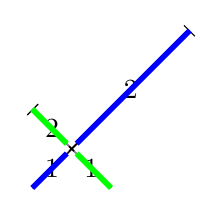
\begin{tikzpicture}
\draw[spath/save=pathA] (0,0) -- (2,2);
\draw[spath/save=pathB] (1,0) -- (0,1);

\tikzset{
  spath/.cd,
  split at intersections={pathA}{pathB},
  get components of={pathA}\pathAcomponents,
  get components of={pathB}\pathBcomponents,
}

\foreach[count=\k] \cpt in \pathAcomponents {
  \draw[spath/restore=\cpt,-|];
  \node[fill=white, fill opacity=.5, circle, text opacity=1] at (spath cs:{\cpt} .5) {\(\k\)};
}

\foreach[count=\k] \cpt in \pathBcomponents {
  \draw[spath/restore=\cpt,-|];
  \node[fill=white, fill opacity=.5, circle, text opacity=1] at (spath cs:{\cpt} .5) {\(\k\)};
}

\tikzset{
  spath/.cd,
  insert gaps after components={pathA}{5pt}{1},
  get components of={pathA}\pathAcomponents,
  insert gaps after components={pathB}{5pt}{1},
  get components of={pathB}\pathBcomponents,
}

\foreach[count=\k] \cpt in \pathAcomponents {
  \draw[blue, line width=2pt,spath/restore=\cpt];
%  \node[fill=cyan, fill opacity=.5, circle, text opacity=1] at (spath cs:{\cpt} .5) {\(\k\)};
}

\foreach[count=\k] \cpt in \pathBcomponents {
  \draw[green, line width=2pt,spath/restore=\cpt];
%  \node[fill=cyan, fill opacity=.5, circle, text opacity=1] at (spath cs:{\cpt} .5) {\(\k\)};
}


\end{tikzpicture}

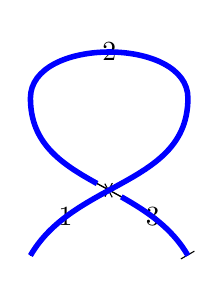
\begin{tikzpicture}
\draw[
  scale=2,
  spath/save=npath,
] (0,0) to[out=60,in=-90] (1,1) to[out=90,in=90] (0,1) to[out=-90,in=120] (1,0);

\tikzset{
  spath/.cd,
  split at self intersections=npath,
  get components of={npath}\npathcomponents,
}

\foreach[count=\k] \cpt in \npathcomponents {
  \draw[spath/restore=\cpt,-|];
  \node[fill=white, fill opacity=.5, circle, text opacity=1] at (spath cs:{\cpt} .5) {\(\k\)};
}

\tikzset{
  spath/.cd,
  insert gaps after components={npath}{10pt}{2},
   join components={npath}{2},
  get components of={npath}\npathcomponents,
}

\foreach[count=\k] \cpt in \npathcomponents {
  \draw[blue, line width=2pt,spath/restore=\cpt];
%  \node[fill=cyan, fill opacity=.5, circle, text opacity=1] at (spath cs:{\cpt} .5) {\(\k\)};
}

\end{tikzpicture}

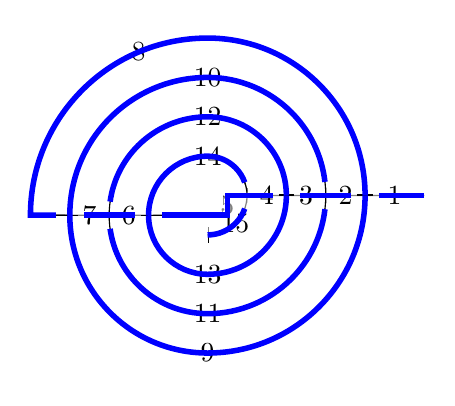
\begin{tikzpicture}
\draw[spath/save=line] (5,0) -- (2.5,0) -- ++(0,-.25) -- ++(-2.5,0)
arc[radius=2.25cm,start angle=180,end angle=90]
arc[radius=2cm,start angle=90, delta angle=-180]
arc[radius=1.75cm,start angle=-90, delta angle=-180]
arc[radius=1.5cm,start angle=90, delta angle=-180]
arc[radius=1.25cm,start angle=-90, delta angle=-180]
arc[radius=1cm,start angle=90, delta angle=-180]
arc[radius=.75cm,start angle=-90, delta angle=-180]
arc[radius=.5cm,start angle=90, delta angle=-180]
;

\tikzset{
  spath/.cd,
  split at self intersections=line,
  get components of={line}\pathcomponents,
}

\foreach[count=\k] \cpt in \pathcomponents {
  \draw[spath/restore=\cpt,-|];
  \node[fill=white, fill opacity=.5, circle, text opacity=1] at (spath cs:{\cpt} .5) {\(\k\)};
}


\tikzset{
  spath/.cd,
  insert gaps after components={line}{10pt}{1,3,5,7,10,11,14},
%  join components={line}{2,4,6,8,9,12,13},
  get components of={line}\pathcomponents,
}

\foreach[count=\k] \cpt in \pathcomponents {
  \draw[blue, line width=2pt,spath/restore=\cpt];
%  \node[fill=cyan, fill opacity=.5, circle, text opacity=1] at (spath cs:{\cpt} .5) {\(\k\)};
}


\end{tikzpicture}


\end{document}


\tikz \calligraphy[copperplate] (0,0) .. controls +(1,-1) and +(-1,1) .. ++(3,0) [this stroke style={light,taper=start}] +(0,0) .. controls +(1,-1) and +(-1,1) .. ++(3,0) [this stroke style={taper,heavy}];

\begin{tikzpicture}
\draw[decorate,decoration={calligraphic brace,amplitude=4mm},ultra thick] (0,0) -- (0,8);
\draw[line width=2pt,decorate,decoration={brace,amplitude=10},line cap=round] (1,0) -- ++(0,8);
\node[anchor=south west,minimum height=8cm,outer sep=0pt,left delimiter=\{] (a) at (2,0) {};
\draw[decorate,decoration={calligraphic straight parenthesis,amplitude=4mm},ultra thick] (3,0) -- ++(0,8);
\draw[decorate,decoration={calligraphic curved parenthesis,amplitude=4mm},ultra thick] (4,0) -- ++(0,8);
\node[anchor=south west,minimum height=8cm,outer sep=0pt,left delimiter=(] (a) at (5,0) {};
\end{tikzpicture}


\begin{tikzpicture}
\draw[save as spath=circular path] (0,0) circle[radius=1cm];
\end{tikzpicture}

\newpage

\SPathPrepare{circular path}

\displaypath{circular path}

\newpage

\begin{tikzpicture}
\draw[save as spath=circular path] (0,0) arc[start angle=0, end angle=360, radius=1cm] -- cycle;
\end{tikzpicture}

\newpage

\SPathPrepare{circular path}

\displaypath{circular path}

\newpage

\begin{tikzpicture}
\draw[save as spath=my path] (0,0) -- (1,1) .. controls +(1,0) and +(-1,0) .. (3,0) -- cycle (4,0) -- (5,1) -- (6,0) -- cycle;
\end{tikzpicture}

\newpage

\SPathPrepare{my path}

\displaypath{my path}

\newpage
\SPathTranslateInto {my path} {translated path} {10pt} {-10pt}

\displaypath{translated path}

\newpage
\SPathWeldInto {my path} {weld path} {translated path}

\displaypath{weld path}

\newpage
\begin{tikzpicture}
\draw[restore spath=my path];
\end{tikzpicture}

\begin{tikzpicture}
\draw[restore spath=weld path];
\end{tikzpicture}
\newpage

\begin{tikzpicture}
\draw[define pen,red,ultra thick] (0,0) -- (.2,.2) (.3,.3) (.4,.4) -- (.6,.6);
\draw[blue,ultra thick] (0,0) .. controls +(1,.5) and +(-1,.5) .. (3,0);
%\draw[shift={(1cm,1cm)},use pen,pen colour=green] (0,0) .. controls +(1,.5) and +(-1,.5) .. (3,0) (4,0) -- (4,1);
\draw[use pen] (0,0) -- (1,.5) -- (2,0);
\draw[use pen] (3,.5) -- (4,0);
\draw[use pen] (5,0) .. controls +(1,.5) and +(-1,.5) .. +(3,0);
\draw[use pen,nib style={1}{pen colour=green}] (9,0) .. controls +(1,.5) and +(-1,.5) .. ++(3,0) .. controls +(1,-.5) and +(-1,-.5) .. ++(3,0);
\end{tikzpicture}

\begin{tikzpicture}
\begin{scope}[every path/.append style={use pen=copperplate,line width=1mm,pen colour=green,taper,taper width=.5mm}]
\draw (0,0) -- (1,.5) -- (2,0);
\draw (3,.5) -- (4,0);
\draw (5,0) .. controls +(1,.5) and +(-1,.5) .. +(3,0);
\draw (9,0) .. controls +(1,.5) and +(-1,.5) .. ++(3,0) .. controls +(1,-.5) and +(-1,-.5) .. ++(3,0);
\end{scope}
\end{tikzpicture}

\begin{tikzpicture}
\draw[use pen=copperplate,taper,stroke style={1}{heavy},light,stroke style={2}{taper start=false}] (0,0) .. controls +(1,.5) and +(-1,-.5) .. ++(3,0) ++(0,0) [this stroke style={pen colour=green}] .. controls +(1,.5) and +(-1,-.5) .. ++(3,0);
\end{tikzpicture}


\end{document}
